\documentclass{article}

% Language setting
% Replace `english' with e.g. `spanish' to change the document language
\usepackage[english]{babel}
\usepackage[utf8]{inputenc}

% Set page size and margins
% Replace `letterpaper' with `a4paper' for UK/EU standard size
\usepackage[a4paper,top=2cm,bottom=2cm,left=3cm,right=3cm,marginparwidth=1.75cm]{geometry}

% Useful packages
\usepackage{amsmath, amssymb, amsthm}
\usepackage{geometry}
\usepackage{graphicx}
\usepackage{physics} % For nicer derivatives, etc.
\usepackage{enumitem}
\usepackage{hyperref} % For clickable links
\usepackage{xcolor}
\usepackage{fancyhdr} % For header and footer
\usepackage{tikz}

%--- Theorem, Definition, etc. Environments ---
\theoremstyle{definition}
\newtheorem{definition}{Definition}[section]
\newtheorem{example}{Example}[section]

\theoremstyle{plain}
\newtheorem{theorem}{Theorem}[section]
\newtheorem{lemma}{Lemma}[section]
\newtheorem{proposition}{Proposition}[section]
\newtheorem{corollary}{Corollary}[section]

\theoremstyle{remark}
\newtheorem{remark}{Remark}[section]

\renewcommand{\qedsymbol}{$\blacksquare$} % Define the end of proof symbol

% --- Header and Footer ---
\pagestyle{fancy}
\fancyhf{} % Clear header and footer
\renewcommand{\headrulewidth}{0.4pt} % Set header line thickness
\renewcommand{\footrulewidth}{0.4pt} % Set footer line thickness
\fancyhead[C]{\footnotesize Lecture \thesection: Introduction} % Center Header with section
\fancyhead[R]{\footnotesize \today}  % Right Header
\fancyfoot[C]{\footnotesize \thepage} % Center Footer - page number

%--- Color Definitions ---
\definecolor{myblue}{rgb}{0.1, 0.4, 0.7}
\definecolor{mygreen}{rgb}{0.1, 0.7, 0.1}

\hypersetup{colorlinks=true,
            linkcolor=myblue,
            citecolor=mygreen,
            urlcolor=myblue}

\title{Classical Mechanics (McGill University)}
\author{Alexander Maloney, Zeyu Li}
\date{\today}

\begin{document}

\maketitle

\setcounter{section}{0}

\section{Lecture 1: Introduction, Degrees of Freedom, and Lagrangian Dynamics}

\subsection{Introduction}

The objective of this course is to develop a deep understanding of classical dynamical systems through the lens of Lagrangian mechanics. We will explore how systems evolve over time by transitioning from Newtonian formulations to a more elegant and generalized Lagrangian framework.

\subsubsection*{Coordinate Systems}

\paragraph{Cartesian Coordinates.}
In Cartesian coordinates, the position, velocity, and acceleration of a particle are given by:
\begin{equation}
    \begin{aligned}
        \mathbf{r} & = (x, y, z)         \\
        \mathbf{v} & = \dot{\mathbf{r}}  \\
        \mathbf{a} & = \ddot{\mathbf{r}}
    \end{aligned}
\end{equation}

\paragraph{Polar Coordinates.}
For a planar motion described in polar coordinates $(r,\theta)$, the time derivatives of the unit vectors are:
\begin{equation}
    \begin{aligned}
        \frac{d\hat{\mathbf{e}}_r}{dt}      & = \dot{\theta}\,\hat{\mathbf{e}}_\theta \\
        \frac{d\hat{\mathbf{e}}_\theta}{dt} & = -\dot{\theta}\,\hat{\mathbf{e}}_r
    \end{aligned}
\end{equation}
The position and velocity in polar coordinates become:
\begin{equation}
    \begin{aligned}
        \mathbf{r} & = (r, \theta) \\
        \mathbf{v} & = \dot{\mathbf{r}} = \frac{d}{dt}\Bigl(r\,\hat{\mathbf{e}}_r\Bigr)
        = \dot{r}\,\hat{\mathbf{e}}_r + r\,\dot{\theta}\,\hat{\mathbf{e}}_\theta \\
        \mathbf{a} & = \ddot{\mathbf{r}}
    \end{aligned}
\end{equation}

\paragraph{Three-Dimensional Space.}
For a single particle moving in three-dimensional space, its state is described as:
\begin{equation}
    \begin{aligned}
        \mathbf{r} & = (x_1, x_2, x_3)   \\
        \mathbf{v} & = \dot{\mathbf{r}}  \\
        \mathbf{a} & = \ddot{\mathbf{r}}
    \end{aligned}
\end{equation}

\paragraph{Spherical Coordinates.}
In spherical coordinates, where the position is expressed as $(r,\theta,\phi)$, the velocity is given by:
\begin{equation}
    \begin{aligned}
        \mathbf{r} & = (r,\theta,\phi) \\
        \mathbf{v} & = \dot{\mathbf{r}} = \dot{r}\,\hat{\mathbf{r}} + r\,\dot{\theta}\,\hat{\boldsymbol{\theta}} + r\,\dot{\phi}\,\sin\theta\,\hat{\boldsymbol{\phi}}
    \end{aligned}
\end{equation}

\subsection{Degrees of Freedom and Generalized Coordinates}

Newton's second law, $\mathbf{F} = m\mathbf{a}$, governs the dynamics of a particle. However, when dealing with complex systems—especially those subject to constraints—Newtonian mechanics may become unwieldy. Lagrangian mechanics provides an efficient and systematic approach by using \emph{generalized coordinates}.

\begin{definition}[Generalized Coordinates]
    Generalized coordinates are a set of parameters used to represent the state of a system in a configuration space.  If the coordinates are independent of one another, the number of independent generalized coordinates is defined by the number of degrees of freedom of the system.
\end{definition}

\begin{definition}[Degrees of Freedom]
    The degrees of freedom (DOF) of a system refer to the number of independent parameters required to specify its configuration.
\end{definition}

For a system of $M$ particles in three-dimensional space, without constraints, each particle has 3 degrees of freedom, giving a total of $3M$. When $N$ independent constraints are present, the effective number of degrees of freedom is reduced to:
\begin{equation}
    \text{DOF} = 3M - N.
\end{equation}

\subsubsection*{Examples of Constrained Systems}

In figure \ref{fig:1-1-1}, we have:

\begin{itemize}
    \item \textbf{Two particles connected by a rod:}
          The distance between the two particles is fixed, hence:
          \begin{equation}
              \text{DOF} = 3 \times 2 - 1 = 5.
          \end{equation}

    \item \textbf{Four particles connected by rods with fixed angles:}
          With three constraints due to fixed lengths and an additional three constraints from fixed angles, the system reduces to the degrees of freedom of a rigid body:
          \begin{equation}
              \text{DOF} = 3 \times 4 - 3 \text{ (length constraints)} - 3 \text{ (angular constraints)}
              = 6,
          \end{equation}
          which corresponds to 3 translational and 3 rotational degrees of freedom.

    \item \textbf{Three particles connected by rods with one unfixed angle:}
          Removing one constraint results in:
          \begin{equation}
              \text{DOF} = 3 \times 3 - 2 = 7.
          \end{equation}
\end{itemize}

\begin{figure}[ht]
    \centering
    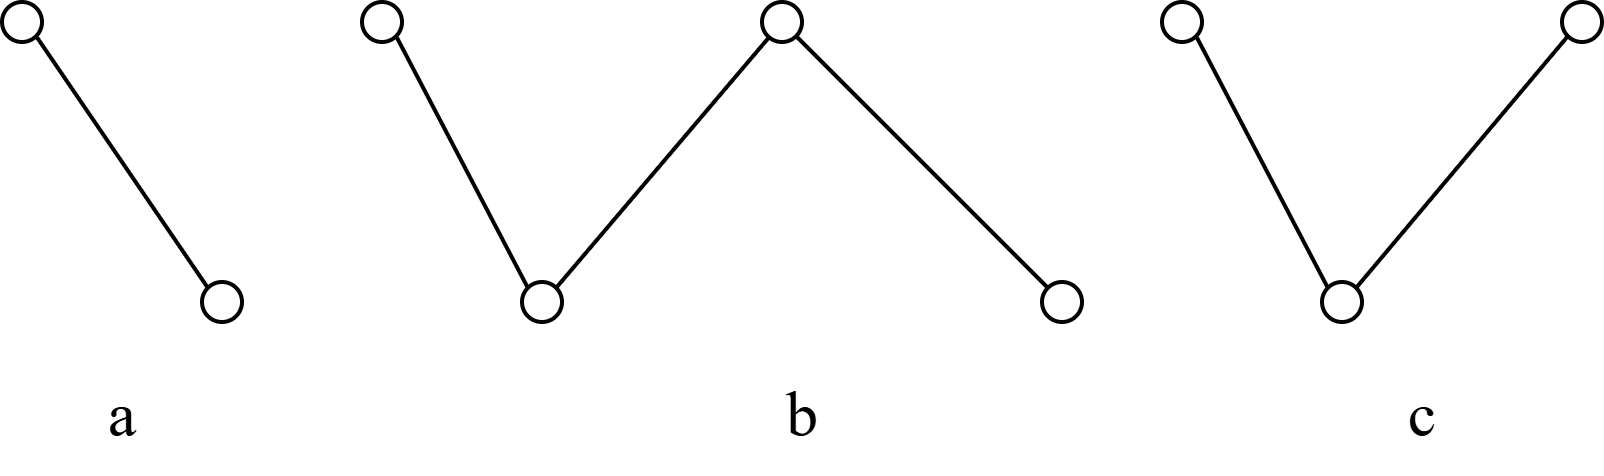
\includegraphics[width=0.8\textwidth]{images/1-1-1.png}
    \caption{Examples of Constrained Systems}
    \label{fig:1-1-1}
\end{figure}

\subsubsection*{The Simple Pendulum}

Consider the simple pendulum depicted in Figure~\ref{fig:1-1-2}. The pendulum's motion is fully described by a single parameter (e.g., the angle $\theta$), hence it has one degree of freedom.

\begin{figure}[ht]
    \centering
    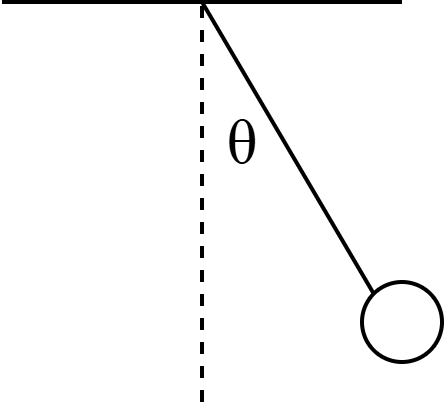
\includegraphics[width=0.3\textwidth]{images/1-1-2.png}
    \caption{Simple Pendulum}
    \label{fig:1-1-2}
\end{figure}

\subsubsection*{Generalized Coordinates for Constrained Systems}

In the context of constrained systems, we introduce a set of generalized coordinates $\{q_i\}$, where $i = 1, 2, \dots, N$, with $N$ being the number of degrees of freedom. The position of each particle in the system can be expressed as:
\begin{equation}
    \mathbf{r}_\alpha = \mathbf{r}_\alpha(q_i, t), \quad \alpha = 1, 2, \dots, M.
\end{equation}
If the equation of constraint contain the time as an explicit variable, then it is referred to as \textbf{rheonomous} constraint; otherwise, it is \textbf{scleronomous}. 

Moreover, if the constraint can be expressed as $f\left(q_1, q_2, \cdots, q_n, t\right)$, where $q_1$, $q_2$, $\cdots$, $q_n$ are the generalized coordinates, without containing velocities and so forth, then it is referred to as \textbf{holonomic} constraint; otherwise, it is \textbf{nonholonomic}.

\begin{figure}[ht]
    \centering
    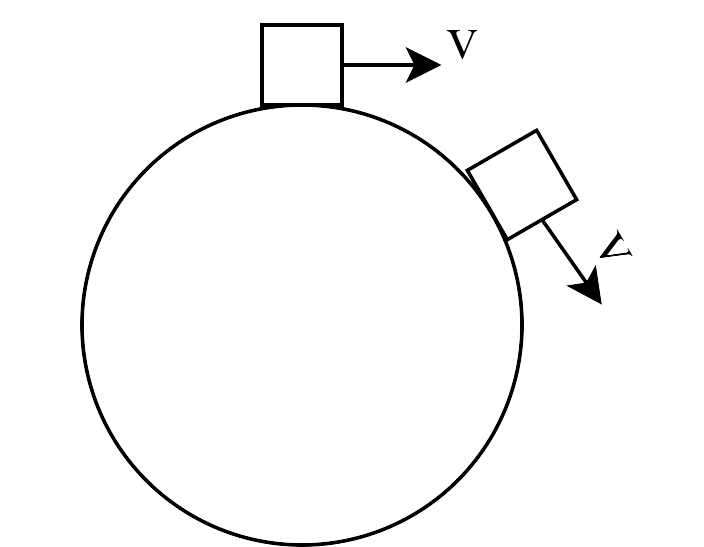
\includegraphics[width=0.3\textwidth]{images/1-1-3.png}
    \caption{Example of a Nonholonomic System}
    \label{fig:1-1-3}
\end{figure}

Nonholonomic systems frequently occur in practice. For example, consider a box moving on the surface of a sphere in figure \ref{fig:1-1-3}: when the box loses contact with the surface, the effective degrees of freedom increase.

\subsection{Lagrangian Mechanics}

Consider a system described by the generalized coordinates $q_i$, where $i = 1, 2, ..., N$ (number of DOF). The positions of the system's parts can be written as $\mathbf{r}_\alpha = \mathbf{r}_\alpha(q_i, t)$. The fundamental problem is to determine the time evolution of these generalized coordinates, $q_i(t)$. These will satisfy a set of $N$ differential equations, known as the \textbf{equations of motion}.

Traditionally, Newton's laws of motion were used, which requires dealing with constraint
forces:

\begin{enumerate}
    \item Determine the force $\mathbf{F}_\alpha$ acting on each part of the system at
          position $\mathbf{r}_\alpha$.
    \item Apply Newton's second law, which gives a system of second-order ordinary
          differential equations (ODEs):

          \begin{equation}
              \mathbf{F}_\alpha = m_\alpha \ddot{\mathbf{r}}_\alpha
          \end{equation}

    \item  Rewrite $\mathbf{r}_\alpha$ in terms of $q_i$. This can be challenging to
          actually implement!
\end{enumerate}

Lagrangian mechanics provides an elegant way to avoid dealing with constraint forces
directly.

Consider an infinitesimal change in position, $\delta \mathbf{r}_\alpha$. The work done
by the force is:

\begin{equation}
    \delta W = \sum_{\alpha} \mathbf{F}_\alpha \cdot \delta \mathbf{r}_\alpha
\end{equation}

A crucial question arises: how much work is done if we change the generalized coordinates
from $q_i$ to $q_i + \delta q_i$? Since $\mathbf{r}_\alpha = \mathbf{r}_\alpha(q_i, t)$,
the variation in position can be written as:

\begin{equation}
    \delta \mathbf{r}_\alpha = \sum_{i} \frac{\partial \mathbf{r}_\alpha}{\partial q_i} \delta q_i
\end{equation}

This assumes that we only consider variations in the generalized coordinates, keeping
$t$ constant. Thus:

\begin{align}
    \delta W & = \sum_{\alpha} \mathbf{F}_\alpha \cdot \left(\sum_{i} \frac{\partial \mathbf{r}_\alpha}{\partial q_i} \delta q_i \right)    \\
             & = \sum_{i} \left(\sum_{\alpha} \mathbf{F}_{\alpha} \cdot \frac{ \partial \mathbf{r}_\alpha}{\partial q_i} \right) \delta q_i
\end{align}

We define the term in the parenthesis to be a \textbf{generalized force}:

\begin{equation}
    F_i = \sum_{\alpha} \mathbf{F}_{\alpha} \cdot \frac{\partial \mathbf{r}_\alpha}{\partial q_i}
\end{equation}

Here, $F_i$ is the generalized force associated with the generalized coordinate $q_i$. It effectively represents the force component in the "allowed" direction defined by the variation in $q_i$.

Now let's consider the kinetic energy of a constrained system:

\begin{align}
    T & = \frac{1}{2} \sum_{\alpha} m_\alpha \dot{\mathbf{r}}_\alpha \cdot \dot{\mathbf{r}}_\alpha \\
      & = T(q_i, \dot{q_i}, t)                                                                     \\
\end{align}

where,

\begin{align}
    \mathbf{r}_\alpha       & = \mathbf{r}_\alpha(q_i, t)                                                                                        \\
    \dot{\mathbf{r}}_\alpha & = \sum_i \frac{\partial \mathbf{r}_\alpha}{\partial q_i} \dot{q_i} + \frac{\partial \mathbf{r}_\alpha}{\partial t}
\end{align}

Note that from the expression above, we have

\begin{equation}
    \frac{\partial \dot{\mathbf{r}}_\alpha}{\partial \dot{q_i}} = \frac{\partial \mathbf{r}_\alpha}{\partial q_i}
\end{equation}

We can compute the partial derivatives of the kinetic energy:

\begin{align}
    \frac {\partial T}{\partial q_i}       & = \sum_\alpha m_\alpha \dot{\mathbf{r}}_\alpha \cdot \frac{\partial \dot{\mathbf{r}}_\alpha}{\partial q_i}                                                                                                            \\
    \frac {\partial T}{\partial \dot{q_i}} & = \sum_\alpha m_\alpha \dot{\mathbf{r}}_\alpha \cdot \frac{\partial \dot{\mathbf{r}}_\alpha}{\partial \dot{q_i}} = \sum_\alpha m_\alpha \dot{\mathbf{r}}_\alpha \cdot \frac{\partial \mathbf{r}_\alpha}{\partial q_i} \\
\end{align}

Now, let's compute the time derivative of $\frac {\partial T}{\partial \dot{q_i}}$:

\begin{align}
    \frac{d}{dt} \left(\frac {\partial T}{\partial \dot{q_i}}\right) & = \sum_\alpha m_\alpha \left(\ddot{\mathbf{r}}_\alpha \cdot \frac{\partial \mathbf{r}_\alpha}{\partial q_i} + \dot{\mathbf{r}}_\alpha \cdot \frac{\partial \dot{\mathbf{r}}_\alpha}{\partial q_i}\right) \\
                                                                     & = \sum_\alpha \mathbf{F}_\alpha \cdot \frac{\partial \mathbf{r}_\alpha}{\partial q_i} + \frac{\partial T}{\partial q_i}                                                                                  \\
                                                                     & = F_i + \frac{\partial T}{\partial q_i}                                                                                                                                                                  \\
\end{align}

Therefore, we have the following important relation:

\begin{equation}
    F_i = \frac{d}{dt} \left(\frac {\partial T}{\partial \dot{q_i}}\right) - \frac{\partial T}{\partial q_i}
\end{equation}

If we know the kinetic energy $T(q_i, \dot{q}_i, t)$, we can obtain the generalized force
without directly calculating constraint forces! This provides a powerful generalization
of $\mathbf{F} = m\mathbf{a}$ to a generic degree of freedom.
\section{Lecture 2: Lagrangian Mechanics, Euler-Lagrange Equation \& Hamiltonians}

\subsection{Lagrangian Mechanics \& Euler-Lagrange Equation}

Consider the following simplification: consider the case where the force $\mathbf{F}_\alpha$ is conservative. A force $\mathbf{F}_\alpha$ is \textbf{conservative} if:

\[
    \oint \mathbf{F}_\alpha \, d\mathbf{r}_\alpha = 0
\]

i.e., the work done to change the state of the system is independent of the path through the space of $\mathbf{r}_\alpha$. For a conservative force, 

\begin{align*}
    \mathbf{F}_\alpha &= \mathbf{\nabla}_\alpha V(\mathbf{r}_1,\ ...,\ \mathbf{r}_\alpha) \\
    &= - \frac{\partial}{\partial \mathbf{r}_\alpha} V(\mathbf{r}_1,\ ...,\ \mathbf{r}_\alpha)
\end{align*}

And the work done to change the state of the system from $\mathbf{r}_\alpha$ to $\mathbf{r}_\alpha^\prime$ is $V(\mathbf{r}_\alpha^\prime)-V(\mathbf{r}_\alpha)$. In this class, we will mostly consider conservative forces.

Since $\mathbf{r}_\alpha=\mathbf{r}_\alpha(q_i, t)$, we can write $V(\mathbf{r}_\alpha)$ as:

\[
    V(\mathbf{r}_\alpha)=V(q_i, t)
\]

From \textbf{Chain Rule}, we can get:

\[
    \frac{\partial V}{\partial q_i}=\sum_\alpha \frac{\partial V}{\partial \mathbf{r}_\alpha} \frac{\partial \mathbf{r}_\alpha}{\partial q_i}=-\sum_\alpha \mathbf{F}_\alpha \frac{\partial \mathbf{r}_\alpha}{\partial q_i}=-\mathbf{F}_i
\]

Then for a conservative force, we can get:

\[
    \frac{d}{dt} (\frac{\partial T}{\partial \dot{q}_i}) - \frac{\partial T}{\partial q_i} = -\frac{\partial V}{\partial q_i}
\]

Since $V$ is not a function of $q_i$, we can get:

\[
    \frac{\partial V}{\partial \dot{q}_i}=0
\]

So we can rewrite the EOM above by defining \textbf{Lagrangian} $L=T-V$, $L=L(q_i, \dot{q}_i, t)$

\[
    \frac{d}{dt} (\frac{\partial L}{\partial \dot{q}_i}) - \frac{\partial L}{\partial q_i} = 0
\]

This EOM is called \textbf{Euler-Lagrange Equation}. We can see that for a general dynamic system, if we can compute $L=T-V$, then we can find the equations of motion!

This is a set of $N$ differential equations, one for each DOF, where $N$ is the total number of DOF. Typically, these are $2^{\text{nd}}$ order ODEs for $q_i$.

To summarize, given a system of M parts and N degrees of freedom, it is advised to follow the following steps:

\begin{enumerate}
    \item Identify some dynamic variables $q_i$, and write down $\mathbf{r}_\alpha=\mathbf{r}_\alpha(q_i, t)$, where $\alpha=1,2,...,M$, $i=1,2,...,N$.
    \item Compute $T=\sum_\alpha \frac{1}{2} m_\alpha \dot{\mathbf{r}}_\alpha \cdot \dot{\mathbf{r}}_\alpha$ as a function of $q_i$.
    \item Compute $V=V(\mathbf{r}_\alpha)=V(q_i, t)$.
    \item Let $L=T-V$.
    \item We can get equations of motion: $\frac{d}{dt} (\frac{\partial L}{\partial \dot{q}_i}) - \frac{\partial L}{\partial q_i} = 0$.
\end{enumerate}

\begin{figure}[ht]
  \centering
  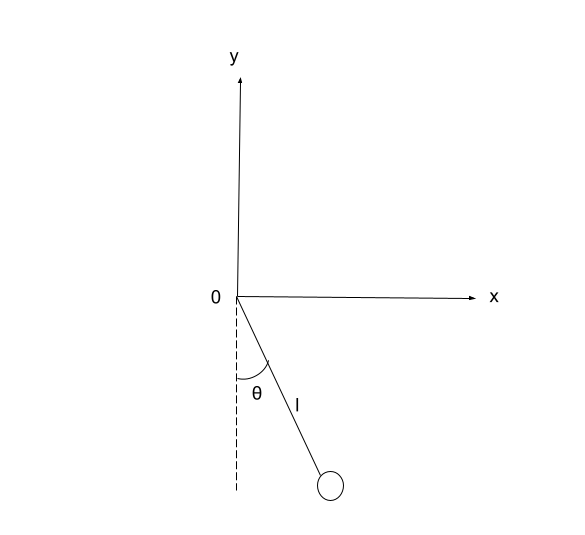
\includegraphics[width=0.8\textwidth]{images/2-1-1.png}
  \caption{Pendulum Example}
  \label{fig:2-1-1}
\end{figure}

For example, let's take a look at the pendulum in Figure \ref{fig:2-1-1}.

\begin{align*}
    x &= l \sin{\theta} \\
    y &= -l \cos{\theta} \\
\end{align*}

So we can get:

\begin{align*}
    \dot{x} &= l \cos{\theta} \cdot \dot{\theta} \\
    \dot{y} &= l \sin{\theta} \cdot \dot{\theta} \\
\end{align*}

So the kinetic energy can expressed as:

\[
    T=\frac{1}{2} m \left(\dot{x}^2+\dot{y}^2\right) = \frac{1}{2} ml^2\dot{\theta}^2
\]

The potential energy is:

\[
    V=-mgy=-mgl\cos{\theta}
\]

\[
    L=\frac{1}{2}ml^2\dot{\theta}^2+mgl\cos{\theta}
\]

From \textbf{Euler-Lagrange Equation} we can get:

\[
    ml^2\Ddot{\theta}+mgl\sin{\theta}=0
\]

This is exactly the same as we get using Newton's Law!

\subsection{Hamiltonian Mechanics}

The Lagrangian Mechanics is conceptually useful. But what if we step further? We have dynamic variables $q_i$, $L(q, q_i, t)$, so we define the \textbf{Hamiltonian} as $H=\sum_i \dot{q_i} \frac{\partial L}{\partial \dot{q_i}} - L$.

\[
    \frac{dH}{dt}=\sum_i \left(\Ddot{q_i} \frac{\partial L}{\partial \dot{q_i}} + \dot{q_i} \frac{d}{dt} \left(\frac{\partial L}{\partial \dot{q_i}}\right)\right) - \sum_i \left(\frac{\partial L}{\partial q_i} \dot{q_i} + \frac{\partial L}{\partial \dot{q_i}} \Ddot{q_i} \right) - \frac{\partial q_i}{\partial t}
\]

We know:

\[
    \frac{\partial L}{\partial q_i}=\frac{d}{dt} \left(\frac{\partial L}{\partial \dot{q_i}}\right)
\]

So we can get the following equation:

\[
    \frac{dH}{dt}=-\frac{\partial L}{\partial t}
\]

The total time derivative of $H$ is the explicit time derivative of $L$! If $L$ has no explicit time dependence, then we can get:

\[
    \frac{dH}{dt}=0
\]

i.e., $H$ is conserved.

So what is the \textbf{Hamiltonian}? If the constraints are time independent,

\[
    \mathbf{r}_\alpha=\mathbf{r}_\alpha (q_i)
\]

Then we can get

\[
    T=\frac{1}{2} \sum_\alpha m_\alpha \dot{\mathbf{r}_\alpha} \cdot \dot{\mathbf{r}_\alpha}
\]

\[
    \frac{\partial L}{\partial \dot{q_i}} = \frac{\partial T}{\partial \dot{q_i}} = \sum_\alpha m_\alpha \dot{\mathbf{r}}_\alpha \cdot \frac{\partial \dot{\mathbf{r}}_\alpha}{\partial \dot{q_i}} = \sum_\alpha m_\alpha \dot{\mathbf{r}}_\alpha \cdot \frac{\partial \mathbf{r}_\alpha}{\partial q_i}
\]

\begin{align*}
    \sum_i \dot{q_i} \frac{\partial L}{\partial q_i} &= \sum_i \dot{q_i} \left(\sum_\alpha m_\alpha \dot{\mathbf{r}}_\alpha  \frac{\partial \mathbf{r}_\alpha}{\partial q_i}\right) \\
    &= \sum_\alpha m_\alpha \dot{\mathbf{r}}_\alpha \left(\sum_i \frac{\partial r_\alpha}{\partial q_i} \dot{q_i}\right) \\
    &= \sum_\alpha m_\alpha \dot{\mathbf{r}}_\alpha \cdot \dot{\mathbf{r}}_\alpha \\
    &= 2T
\end{align*}

So we can get:

\begin{align*}
    H &= \sum_i \dot{q_i} \frac{\partial L}{\partial q_i} - L \\
    &= 2T - \left(T - V\right) \\
    &= T + V \\
\end{align*}

So $H$ is the total energy of the system (in many cases)!

We can get the following conclusions from the analysis above:

\begin{enumerate}
    \item If the \textbf{Lagrangian} $L$ is time independent, then the total energy of the system is conserved.
    \item If the \textbf{Lagrangian} $L$ is time independent, the system has time translation symmetry.
\end{enumerate}

So conserved energy is equivalent to time translation symmetry.

\begin{definition}[Noether's theorem]
    Every continuous symmetry of the action of a physical system with conservative forces has a corresponding conservation law.
\end{definition}

Let's look at another example of \textbf{Noether's theorem}: Imagine $L(q_i, \dot{q_i}, t)$ is 
independent of $q_i$ (although it could depend on $q_i$). In this way, we can represent 
$L=L(\dot{q_i}, t)$, so we can get:

\[
    \frac{d}{dt} \left(\frac{\partial L}{\partial \dot{q_i}}\right) = 0
\]

So $\frac{\partial L}{\partial \dot{q_i}}$ is conserved. This is the \textbf{momentum}!

\begin{definition}[Momentum]
    The \textbf{momentum} $p_i$ conjugated to $q_i$ is defined as $\frac{\partial L}{\partial \dot{q_i}}$.
    This momentum is conserved if the Lagrangian $L$ is independent of the coordinate $q_i$.
\end{definition}

At last, let's take a look at a particle moving in a circle. We have the following equations of motion:

\begin{align*}
    x&=R\cos(\theta)\\
    y&=R\sin(\theta)\\
\end{align*}

So we can get:

\begin{align*}
    \dot{x}&=-R\sin(\theta)\dot{\theta}\\
    \dot{y}&=R\cos(\theta)\dot{\theta}\\
\end{align*}

\[
    L = T = \frac{1}{2} m (\dot{x}^2+\dot{y}^2) = \frac{1}{2} m R^2 \dot{\theta}^2
\]

$L$ is independent of $\theta$.

\[
    p_\theta =  m R^2 \dot{\theta} = \text{angular momentum}
\]

In summary, a linear translation symmetry leads to conservation of momentum, a 
rotational symmetry leads to conservation of angular momentum, a time translation
symmetry leads to conservation of energy. % Example if you add more lecture files, 
%\section{Lecture 3: Action Principle \& Calculus of Variations}

\subsection{Action Principle}

For beginning, let's recall the Fermat's Principle.

\begin{definition}[Fermat's Principle]
    Light travels along the shortest path between two points.
\end{definition}

Precisely speaking, the length of a curve $L = \int ds \sqrt{\left(\frac{dx}{ds}\right)^2 + \left(\frac{dy}{ds}\right)^2}$
will be minimized for the trajectory of light.

Then we need to ask the following question: does every mechanical system obey a 
minimization principle of this sort? The answer is yes. So let's consider the set of all
possible paths $q_i\left(t\right)$ that a system could take through configuration space.

For a given path $q_i\left(t\right)$, we define the action of this path as
$S[q_i\left(t\right)]$.

\[
    s[q_i\left(t\right)] = \int_{t_\text{initial}}^{t_\text{final}} L\left(q_i, \dot{q}_i, t\right) dt
\]

The path that a mechanical system takes through configuration space (nearly space of $q_i$)
"minimizes" $S[q_i\left(t\right)]$ (not global, only local extremum). This is called the
\textbf{Least Action Principle}, or alternatvely, \textbf{Hamiltonian's Principle}. 
$S[q_i\left(t\right)]$ is a function of a function, so it is called a \textbf{functional}.
For functionals, we use square brackets $[f]$ to denote the dependence rather than curve bracket
$f\left(x\right)$.

 % Example if you add more lecture files, 

\end{document}